\pagenumbering{arabic}

\def\papertitle{Title of paper}
% \def\authors{}
% \def\journal{Some Journal}
% \def\doi{12345}
% Define title defaults if not defined by user
\providecommand{\lettertitle}{Author Response to Reviews of}
\providecommand{\papertitle}{Title}
\providecommand{\authors}{Authors}
\providecommand{\journal}{Journal}
\providecommand{\doi}{--}

\newgeometry{includeheadfoot,top=20mm, bottom=20mm, footskip=2.5cm}

% Colors
\definecolor{reply}{HTML}{0570b0}

% Table

\renewcommand{\arraystretch}{1.5} % enlarge spacing between rows

\captionsetup[table]{skip=10pt} % enlarge spacing between caption and table

% Section styles

\titleformat{\section}{\normalfont\large}{\makebox[0pt][r]{\bf \thesection.\hspace{4mm}}}{0em}{\bfseries}
\titleformat{\subsection}{\normalfont}{\makebox[0pt][r]{\bf \thesubsection.\hspace{4mm}}}{0em}{\bfseries}
\titlespacing{\subsection}{0em}{1em}{-0.3em} % left before after

% Paragraph styles

\setlength{\parskip}{0.6\baselineskip}%
\setlength{\parindent}{0pt}%

% Quotation styles

\let\oldquote=\quote
\let\endoldquote=\endquote
\renewenvironment{quote}{\begin{fquote}\advance\leftmargini -2.4em\begin{oldquote}}{\end{oldquote}\end{fquote}}

\newenvironment{fquote}
  {\def\FrameCommand{
  \fboxsep=0.6em % box to text padding
  \fcolorbox{black}{white}}%
  % the "2" can be changed to make the box smaller
    \MakeFramed {\advance\hsize-2\width \FrameRestore}
    \begin{minipage}{\linewidth}
  }
  {\end{minipage}\endMakeFramed}

% Table styles

\let\oldtabular=\tabular
\let\endoldtabular=\endtabular
\renewenvironment{tabular}[1]{\begin{adjustbox}{center}\begin{oldtabular}{#1}}{\end{oldtabular}\end{adjustbox}}

\long\def\RC#1\par{\makebox[0pt][r]{{\stepcounter{subsection}}RC\thesubsection:\hspace{4mm}}\color{black} #1\par} %\RC
\WithSuffix\long\def\RC*#1\par{\color{black} #1\par} %\RC*
\long\def\AR#1\par{\makebox[0pt][r]{\color{reply} AR:\hspace{4mm}}{\color{reply}#1}\par\vspace{\baselineskip}} %\AR
\WithSuffix\long\def\AR*#1\par{{\color{reply}#1\par\vspace{\baselineskip}}} %\AR*

%%%
%DIF PREAMBLE EXTENSION ADDED BY LATEXDIFF
%DIF UNDERLINE PREAMBLE %DIF PREAMBLE
\definecolor{RED}{rgb}{1,0,0}\definecolor{BLUE}{rgb}{0,0,1} %DIF PREAMBLE
\providecommand{\DIFadd}[1]{{\protect\color{blue}\uwave{#1}}} %DIF PREAMBLE
\providecommand{\DIFdel}[1]{{\protect\color{red}\sout{#1}}}                      %DIF PREAMBLE
%DIF SAFE PREAMBLE %DIF PREAMBLE
\providecommand{\DIFaddbegin}{} %DIF PREAMBLE
\providecommand{\DIFaddend}{} %DIF PREAMBLE
\providecommand{\DIFdelbegin}{} %DIF PREAMBLE
\providecommand{\DIFdelend}{} %DIF PREAMBLE
%DIF FLOATSAFE PREAMBLE %DIF PREAMBLE
\providecommand{\DIFaddFL}[1]{\DIFadd{#1}} %DIF PREAMBLE
\providecommand{\DIFdelFL}[1]{\DIFdel{#1}} %DIF PREAMBLE
\providecommand{\DIFaddbeginFL}{} %DIF PREAMBLE
\providecommand{\DIFaddendFL}{} %DIF PREAMBLE
\providecommand{\DIFdelbeginFL}{} %DIF PREAMBLE
\providecommand{\DIFdelendFL}{} %DIF PREAMBLE
%DIF END PREAMBLE EXTENSION ADDED BY LATEXDIFF

% Make title
{\Large\bf \lettertitle}\\[1em]
{\huge \papertitle}\\[1em]
%{\authors}\\
%{\it \journal, }\texttt{doi:\doi}\\
\hrule

% Legend
\hfill {RC:} Reviewer Comment,\(\quad\) {\color{reply} AR: Author Response}, \textcolor{black!50!white}{\quad\(⬒\)} Manuscript excerpt


\begin{refsegment}

  \AR{We thank all of the reviewers for their careful review and detailed
    suggestions to improve the manuscript. We believe that we have successfully
    addressed all comments raised by the referees from our initial submission.
    The reviewers' suggestions have significantly strengthened our manuscript
    without changing the overall story.

    To address these comments, we provided X new figure panels and included
    several new data including the following highlights:

  \begin{enumerate}
  \item Newstuff.
  \item More new stuff.
  \end{enumerate}

 Major changes to the manuscript are highlighted in orange.

}

\section{Reviewer \#1}

\RC \rlabel{rtxt:commentHere} I didn't like this.

\AR{We appreciate the reviewer noting the potential of our work and we fixed it
  like you said (\Cref{rfig:wow}). Here, we need to thank the reviewer for the
  comment (although not overdo it), then say what we need to address it. We then
  show the exact location in the text where we addressed it, along with
  additional figures. To do this, we use custom \texttt{\textbackslash{}qc},
  \texttt{\textbackslash{}qp}, and \texttt{\textbackslash{}qps} commands to copy
  (\texttt{\textbackslash{}qc}) and paste (\texttt{\textbackslash{}qp} from
  text, \texttt{\textbackslash{}qps} from supplemental). We also highlight major
  changes with \texttt{\textbackslash{}highLight} (does not work across
  paragraphs, just do another \texttt{\textbackslash{}highLight}) Check
  \texttt{paper.tex} for examples.

\qp{fixed}

\qps{otherFixInSupplemental}

\begin{rfigure}[H]
  \centering
  % Makebox here to actually center.
  \makebox[\textwidth]{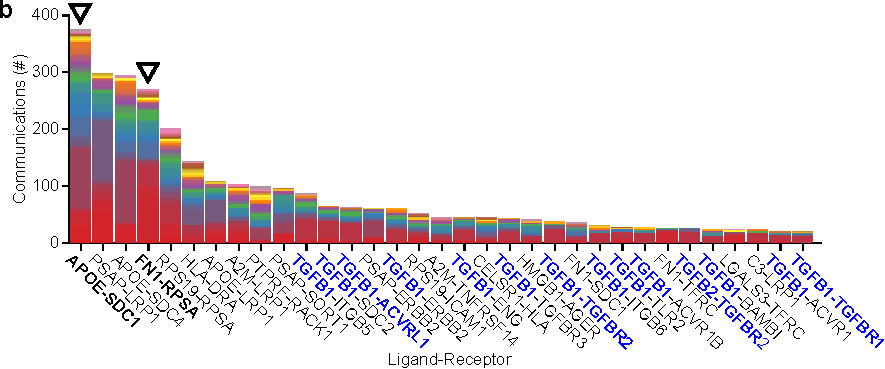
\includegraphics{rebuttal/figures/figure_for_rebuttal.pdf}
  }
  {\phantomsubcaption\label{rfig:wow}}
  \caption{\panel{sub@rfig:wow}, Excerpt from \Cref{fig:astoundingOne}. Minimum
    explanation to understand figure.}
\end{rfigure}

}

\section{Reviewer \#2}

\RC The manuscript reads very well, and the quality of the language is good.

\AR{Thanks. This was noted in R\ref{rtxt:commentHere} too.}

\end{refsegment}

\printbibliography[segment=2]

\end{document}
